\section{Tuning Model Visualization} \label{sec:tm-visualization}
\textbf{TUM (1 page)}
The effect of the best configuration of different tuning parameters can be inspected by comparing different scenarios of the tuning model and explains how similar scenarios appear in closer proximity, while dissimilar scenarios are apart.

The \textit{Forced layout graph} is used to visualize the tuning model result. The graph is constructed based on the JavaScript library D3.js~\cite{bostock2011d3}. It compares scenarios in the tuning model with respect to their similarity and weight. In this context, similarity represents the distance of scenarios in a multi-dimensional tuning space, and weight is the aggregated execution time of \textit{rts's} of a scenario relative to the phase execution time. While similarity is represented by the thickness of the edges between scenarios, the weight is visualized as the size of the circle representing a scenario. Eventually, the distance between scenarios is the result of all forces. The network adapts according to the forces dynamically. 

\begin{figure}
	\begin{mdframed}
	\centering
		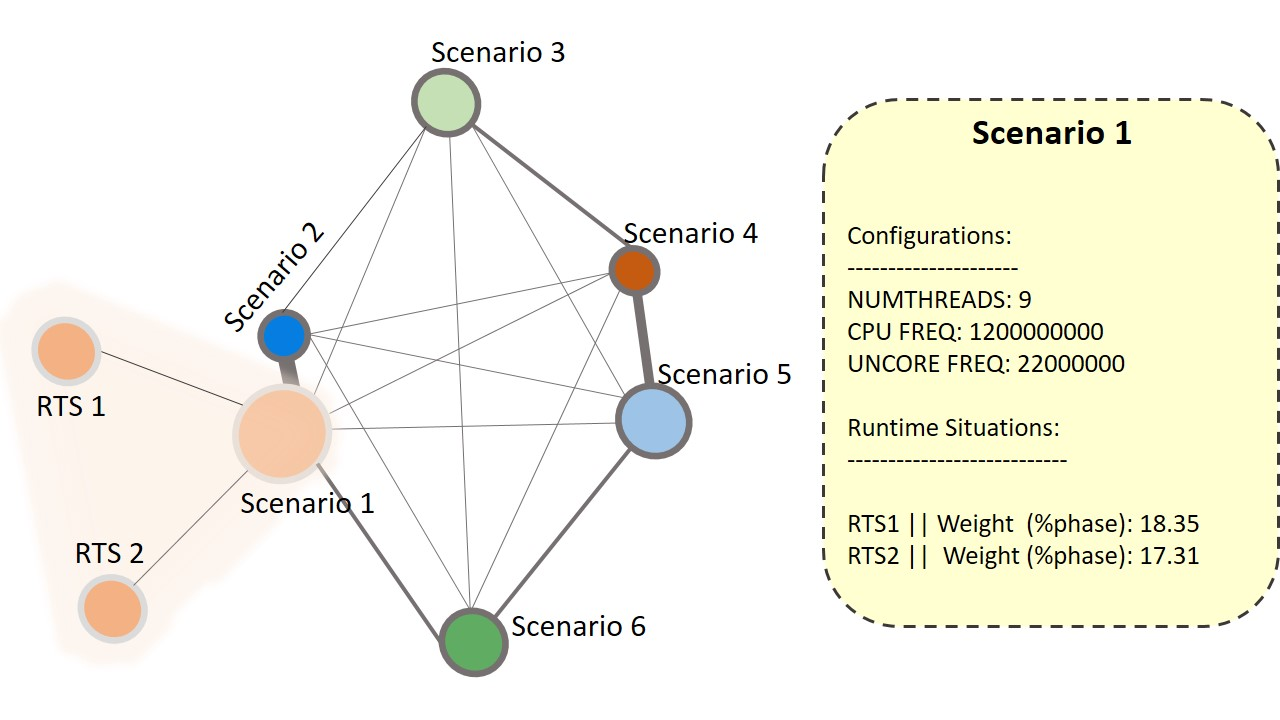
\includegraphics[width=0.60\textwidth]{figures/luleshTM_expand.jpg}
	\end{mdframed}
	\caption{\label{fig:forced-layout-expand}The expanded forced layout of the tuning model of LULESH upon clicking on a scenario node }
\end{figure}

Figure~\ref{fig:forced-layout-expand} shows the tuning model of the LULESH proxy application from the CORAL benchmark suite. The nodes in the figure represent scenarios found in tuning model. Each node is a cluster of \textit{rts's} belonging to it. There are six scenarios in LULESH's tuning model where \texttt{Scenario~1} covers most of the execution time. On the other hand, \texttt{Scenario~2} and \texttt{Scenario~4} are the least significant nodes due to their lowest weights. As the figure shows, \texttt{Scenario~1} and \texttt{Scenario~2} are the most similar scenarios and high thickness of the edge and lowest distance between them affirms that. On the opposite side, \texttt{Scenario~3} and \texttt{Scenario~6} are the most distant dissimilar scenarios.

To investigate each scenario, the user can click on a scenario node of the graph. Upon clicking on a node, the node expands with all the rts nodes of that scenario. A pop over box appears upon hovering on the node which shows the scenario information including rts's with their weight and configurations of the tuning parameters. In this figure, \texttt{Scenario~1} contains two rts's: \texttt{rts 1} and \texttt{rts 2} each representing 18.35\% and 17.31\% weight of the phase respectively. The application tuning parameter is yet to be implemented into ATM.